\chapter{The Probably Approximately Correct Learning Model}
    \section{A Rectangle Learning Game}
    \newcommand{\rectangle}{\mathcal{R}}
    The objective of this game is to learn an unknown \emph{target} (axis-aligned) rectangle \(\rectangle = [a, b] \times [c, d] \subset \reals^2\).
    The player can gain information about \(\rectangle\) only by chosing random points according to some distribution \(\mathcal{D}\) and asking the game whether they are inside \(\rectangle\)

    \begin{figure}
        \begin{center}
                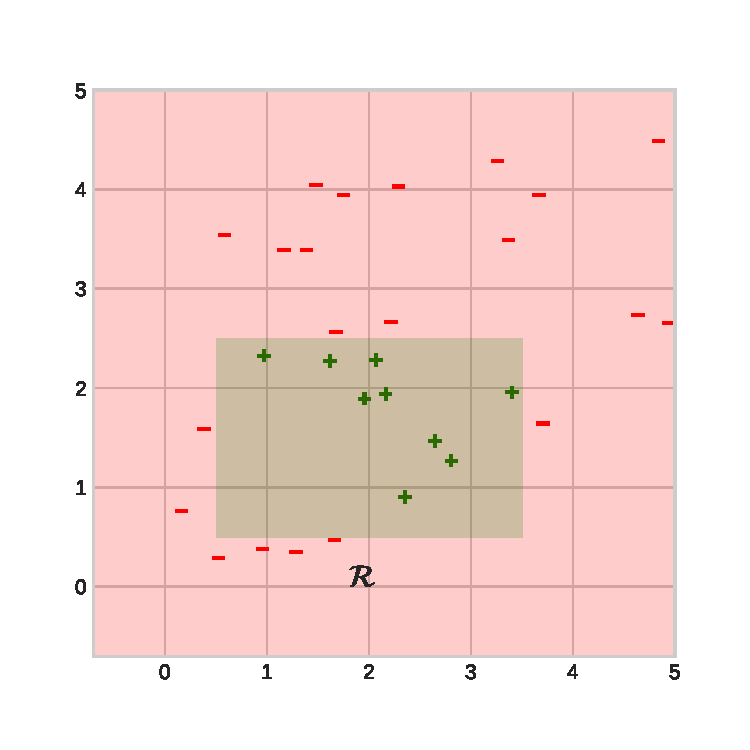
\includegraphics[width=8cm]{traget-and-sample.pdf}
        \end{center}
        \caption{The target triangle along with a labeled sample of points}
    \end{figure}
